\chapter{Introducción}

El presente proyecto constituye un esfuerzo por unir las tecnologías móviles con la astronomía y los instrumentos astronómicos. En los siguientes apartados describiremos las distintas tecnologías o campos de estudio que se verán implicados en el desarrollo posterior:

\begin{itemize}
  \item \itembf{La astronomía.}
  \item \itembf{Instrumental astronómico.}
  \item \itembf{Control de dispositivos astronómicos.}
  \item \itembf{INDI.}
  \item \itembf{Dispositivos móviles.}
\end{itemize}

\section{La Astronomía}

Desde el princpio de los tiempos, el ser humano ha mirado al cielo con incertidumbre, viéndolo como una fuente inagotable de interrogantes sin resolver. En casi todas las religiones antiguas existía la \textbf{``cosmogonía''} que intentaba explicar el origen del universo, ligando este a los elementos mitológicos, dando paso esta a la \textbf{``astronomía''}:

\begin{quote}``\textit{Ciencia que se ocupa del estudio de los cuerpos celestes del universo, incluidos los planetas y sus satélites, los cometas y meteoritos, las estrellas y la materia interestelar, los sistemas de materia oscura, estrellas, gas y polvo llamados galaxias y los cúmulos de galaxias; por lo que estudia sus movimientos y fenómenos ligados a ellos.}''
\newline(\url{https://es.wikipedia.org/wiki/Astronom%C3%ADa})
\end{quote}

\bigskip
 La Astronomía es probablemente la más antigua de las ciencias naturales originándose en la antiguedad en casi todas las culturas humanas. Sus orígenes se pierden en prácticas religiosas de la prehistoria cuyos vestigios se encuentran en numerosos sitios arqueológicos (como Stonehenge) e incorporados todavía en la astrología una disciplina entrelazada con la astronomía y no separada de ella completamente hasta el siglo XVIII en el mundo occidental. La astronomía antigua constituyó las bases del calendario y la medida de periodos temporales como la semana el mes o el año. Los astrónomos antiguos eran capaces de distinguir entre estrellas y planetas dado que las primeras permanecen fijas en sus posiciones relativas mientras que los planetas se mueven una cantidad apreciable de espacio a lo largo de periodos relativamente cortos ( Saturno el más lento de los planetas conocidos en la antigüedad describe un periodo orbital en 29 años). La Astronomía antigua culmina con el desarrollo ordenado del modelo heliocéntrico expuesto en las obras de \textit{Ptolomeo}. Previamente \textit{Aristarco de Samos} había medido las distancias de la Tierra a la Luna y al Sol afirmando como consecuencia de éstas que el Sol era el centro del Universo alrededor del cual giraban los demás planetas incluyendo la Tierra. Otros logros destacados de la época clásica de la astronomía fueron los conseguidos por \textit{Hiparco} quien realizó el primer catálogo estelar y propuso un sistema de clasificación estelar en 6 magnitudes basado en la luminosidad aparente de las diferentes estrellas. La Astronomía en la Europa medieval se produce un oscurantismo en todos los campos del conocimiento incluyendo la astronomía. Ésta permanece preservada en escasas copias de tratados antiguos de la astronomía griega y romana. La astronomía observacional tan sólo se conserva en el mundo árabe.

 \bigskip
 \textit{Tycho Brahe (1546-1601)} introdujo la idea de la precisión de la medida en astronomía e inventó y produjo una gran cantidad de instrumental astronómico previo al telescopio. \textit{Galileo Galilei (1564-1642)} construyó su propio telescopio a partir de un invento holandés y lo utilizó inmediatamente en el estudio astronómico descubriendo los cráteres de la Luna, las lunas de Júpiter y las manchas solares. Sus observaciones tan sólo eran compatibles con el modelo \textbf{copernicano}. Paralelamente \textit{Johannes Kepler} expuso sus famosas \textbf{leyes de Kepler} para el movimiento de los planetas basándo su trabajo en las detalladas observaciones de \textit{Tycho Brahe}.

\bigskip
Una generación más tarde Isaac Newton fue el primer científico que unió la Física con la Astronomía proponiendo que las mismas fuerzas que hacían caer los cuerpos sobre la Tierra causaban el movimiento de los planetas y la Luna. Utilizando su Ley de la gravedad las leyes de Kepler resultan inmediatamente explicadas. Newton también descubrió que la Luz blanca del Sol está descompuesta en diferentes colors, un hecho importantísimo para el futuro desarrollo de la astronomía.

\bigskip
La \textbf{astronomía} es una de las pocas ciencias en las que los aficionados aún puden desempeñar un papel activo, especialmente en el descubirmientos y seguimiento de fenómenos. Es por ello que existe una gran variedad de \textbf{herramientas} e \textbf{instrumental astronómico} que permiten a cualquier persona obervar el universo.

\newpage
\section{Instrumental Astronómico}

Existe una gran variedad de \textbf{instrumental astronómico} en la actualidad. A continuación se describen las familias más importantes.

\subsection{Telescopios}

\begin{quote}``\textit{El telescopio es un instrumento óptico que permite ver objetos lejanos con mucho más detalle que a simple vista al captar radiación electromagnética, tal como la luz.}''
\newline(\url{https://es.wikipedia.org/wiki/Telescopio})
\end{quote}

\begin{figure}[!ht]
  \begin{center}
  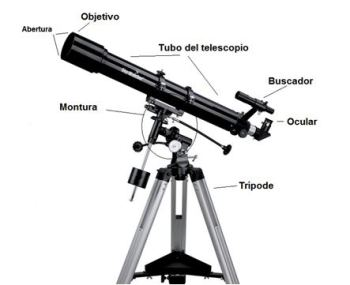
\includegraphics[width=1\textwidth]{../images/telescopio.jpg}
  \caption{Telescopio (\url{https://josevicentediaz.files.wordpress.com}).}
  \label{fig:diag_scrum}
  \end{center}
\end{figure}

\bigskip
Hace cuatro siglos nació un invento que habría de redefinir nuestro lugar en el universo. Tachado en su momento como el instrumento más diabólico de la historia, el telescopio sacudió la sociedad hasta las raíces. Al alzar los ojos al cielo nos convencimos de que éramos el centro de la creación, y había razones para ello: desde nuestra perspectiva, todo parece girar en torno a la Tierra

\bigskip
Los fabricantes de vidrio sabían desde la antigüedad que una esfera de vidrio podía aumentar imágenes, pero tuvieron que pasar siglos antes de que alguien ensamblara dos lentes en un tubo y mirara a través de ellas. Señalar la fecha, lugar y autor exactos de su invención es controvertido. Los holandeses se inclinan por el 2 de octubre de 1608, el día en que \textit{Hans Lippershey} patentó un instrumento llamado \textbf{kijker}, que significa mirador. Un moledor de vidrio holandés aseguraba haber inventado un aparato similar, pero el primero en patentarlo fue \textit{Lippershey}. Como era alemán, vivía en Holanda y registró la patente en Bélgica, más de un país ha pugnado por el honor de su autoría. Sin embargo, como dijo \textit{Darwin}:
\begin{quote}``\textit{en la ciencia el crédito es del que convence al mundo y no del primero en tener la idea}''
\newline(\textbf{Charles Darwin})
\end{quote}
Por eso la gloria se la llevó Italia, ya que fueron las mejoras que introdujo \textit{Galileo} las que permitieron usar el aparato como instrumento astronómico. El diseño de \textit{Galileo} consistía en una lente convexa para el objetivo y otra cóncava en el ocular. En 1611 el alemán \textit{Johannes Kepler} fue el primero en usar dos lentes convexas que enfocaban los rayos en un mismo punto. La configuración de \textit{Kepler} aún se usa en binoculares y cámaras fotográficas modernas y es la base del telescopio refractor.

\bigskip
Tras la muerte de \textit{Galileo}, fue \textit{Isaac Newton} quien nos dio una nueva imagen del universo que sobrevivió 250 años hasta la llegada de \textit{Albert Einstein}.

\begin{quote}``\textit{Si he logrado ver más lejos ha sido porque me he subido a hombros de gigantes}''
\newline(\textbf{Isaac Newton})
\end{quote}

Y así, sobre la herencia de \textit{Galileo}, \textit{Newton} inventó el \textbf{telescopio reflector}, que es la base de los actuales. La innovación consistía en usar espejos en lugar de lentes para enfocar la luz y formar imágenes. Entonces el universo se nos abrió en todo su esplendor.

\subsection{Cámaras CCD}

Un dispositivo de carga acoplada (en inglés \textbf{Charge-Coupled Device}, conocido también como \textbf{CCD}), es un circuito integrado que contiene un número determinado de condensadores enlazados o acoplados. Bajo el control de un circuito interno, cada condensador puede transferir su carga eléctrica a uno o a varios de los condensadores que estén a su lado en el circuito impreso.

\bigskip
\begin{figure}[!ht]
  \begin{center}
  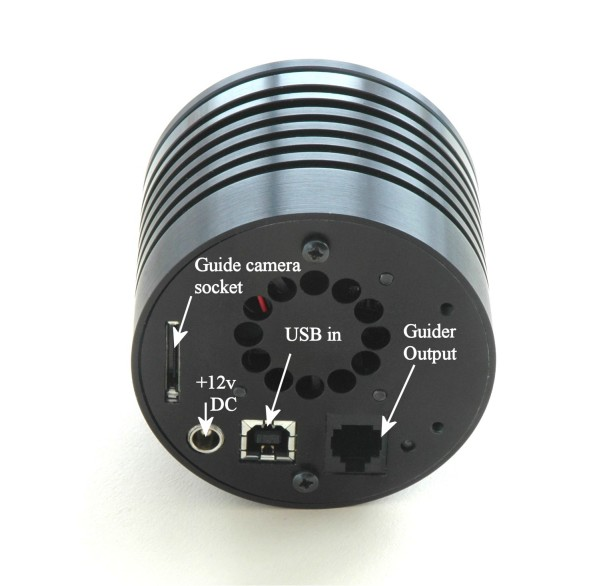
\includegraphics[width=1\textwidth]{../images/ccd.jpg}
  \caption{Cámara CCD (\url{http://www.lunatico.es/}).}
  \label{fig:diag_scrum}
  \end{center}
\end{figure}

\bigskip
El \textbf{CCD} se inventó a finales delos 60 por investigadores de \textbf{Bell Laboratories}. Originalmente se concibió como un nuevo tipo de memoria de ordenador pero pronto se observó que tenía muchas más aplicaciones potenciales tales como el proceso de señales y sobretodo la captación de imagen, esto último debido a la sensibilidad a la luz que presenta el silicio.

\bigskip
El sensor \textbf{CCD} de una cámara digital es como el motor de un coche, es la pieza principal. En su forma más elemental, el \textbf{CCD} es como un ojo electrónico que recoje la luz y la convierte en una señal eléctrica. Tienen dos diferencias básicas con los fotomultiplicadores:

\bigskip
Los sensores \textbf{CCD} son de menor tamaño y están construidos de semiconductores lo que permite la integración de millones de dispositivos sensibles en un solo chip.
La eficiencia cuóntica de los \textbf{CCD} (sensibilidad) es mayor para los rojos. Los fotomultiplicadores son más sensibles a los azules.

\bigskip
Físicamente, un \textbf{CCD} es una malla muy empaquetada de electrodos de polisilicio colocados sobre la superficie de un chip. Al impactar los fotones sobre el silicio se generan electrones generados que pueden guardarse temporalemte. Periódicamente se lee el contenido de cada pixel haciendo que los electrones se desplacen físicamente desde la posición donde se originaron (en la superficie del chip), hacia el amplificador de señal con lo que se genera una corriente eléctrica que será proporcional al número de fotones que llegaron al pixel. Para coordinar los periodos de almacenamiento (tiempo de exposición) y vaciado del pixel (lectura del pixel) debe existir una fuente eléctrica externa que marque el ritmo de almacenamiento-lectura: el reloj del sistema. La forma y amplitud de reloj son críticas en la operación de lectura del contenido de los pixeles.

\bigskip
Al tratarse el \textbf{CCD} de un dispositivo semiconductor, técnicamente es posible implementar en él todas las funciones electrónicas de un sistema de captación de imagen, pero esto no es rentable económicamente y por tanto se implementa en otros chips esternos al \textbf{CCD}: la mayoría de \textbf{CCD} de cámaras tienen varios chips (de tres a ocho).

\bigskip
La necesidad de usar chips distintos implica dos desventajas importantes; la necesidad de voltajes múltiples de abastecimiento de los chips y un gran consumo de potencia de todo el sistema electrónico.

\subsection{Monturas}

La montura de un telescopio es la parte mecánica que une el trípode o base al instrumento óptico. Existen varios tipos de monturas, algunas muy simples, otras mas complejas, incluso con correctores electrónicos y dispositivos de localización y seguimiento muy sofisticados (sistenas \textbf{GOTO})

\bigskip
\begin{figure}[!ht]
  \begin{center}
  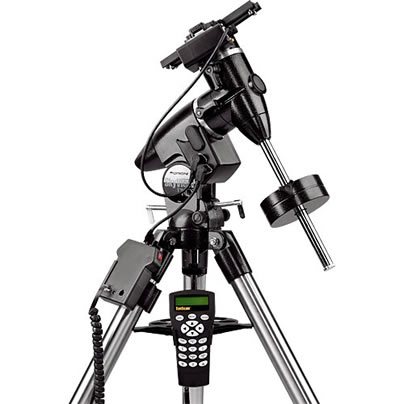
\includegraphics[width=1\textwidth]{../images/montura.jpg}
  \caption{Montura (\url{http://astrofacil.com/}).}
  \label{fig:diag_scrum}
  \end{center}
\end{figure}
http://nimax-img.de/

\bigskip
La montura tiene como objetivo proveer de movimiento controlado al telescopio. Es muy importante la firmeza y suavidad de los movimientos, para que la observación sea confortable y las astrofotografías perfectas. Las monturas se clasifican en dos grandes grupos, según los planos de referencia que utilicen (coordenadas).

\bigskip
La más simple es la montura altacimutal, que realiza movimientos horizontales y verticales (acimut y altura, respectivamente). Este tipo de diseño lo traen incorporados los telescopios pequeños, por lo general telescopios refractores de uso terrestre, dado que su uso es simple, y también varios modelos de equipos automatizados (sistemas \textbf{GOTO})

\bigskip
Le sigue la montura ecuatorial, que utiliza como plano fundamental el ecuador celeste (proyección del ecuador terrestre). Este diseño usa las coordenadas ecuatoriales, ascensión recta (A.R. o R.A.) y declinación (Dec.), que son proyecciones de las coordenadas terrestres longitud y latitud, respectivamente, sobre la esfera celeste.

\bigskip
Existen varios tipos de monturas basados en los dos diseños fundamentales anteriores. La montura \textbf{Dobson} por ejemplo (suelen llamarse telescopios \textit{dobsonianos} a los que la poseen), es un modelo basado en la altacimutal, sin trípode y un telescopio de diseño newtoniano como instrumento de observación. Es muy utilizado por los que desean una gran apertura en reflectores, por ejemplo los que se construyen su propio espejo y no quieran tener grandes gastos en monturas sofisticadas.

\subsection{Rueda portafiltros}

La rueda porta-filtros consiste en un cuerpo, generalmente de aluminio, que en su interior puede alojar varios filtros, normalmente de 1,25" de diámetro. Lo aconsejable es que tenga, al menos, 4 huecos para filtros si queremos hacer astrofotografía con cámaras CCD blanco y negro, puesto que vamos a necesitar el azul, rojo y verde (RGB) y, posiblemente, un filtro para infrarrojos.

\bigskip
\begin{figure}[!ht]
  \begin{center}
  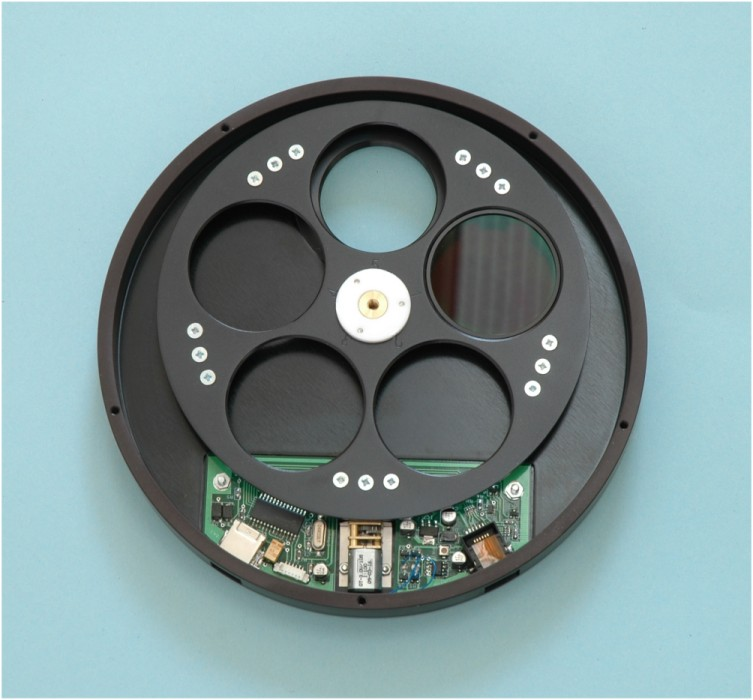
\includegraphics[width=1\textwidth]{../images/portafiltros.jpg}
  \caption{Rueda portafiltros (\url{http://www.lunatico.es/}).}
  \label{fig:diag_scrum}
  \end{center}
\end{figure}

\subsection{Enfocadores}

El \textbf{enfocador} es una pieza fundamental del telescopio. Nos permitirá ver las imágenes formadas tras la reflexión de la luz en el espejo primario y su desviación por el espejo secundario. Para verlas necesitaremos un juego de oculares. La longitud focal de los oculares combinada con la longitud focal de nuestro telescopio nos dará el número de aumentos total del sistema. Dichos oculares están montados en el \textbf{enfocador}, un dispositivo móvil que permitirá mover la posición vertical del ocular para enfocar adecuadamente la imagen.

\bigskip
\begin{figure}[!ht]
  \begin{center}
  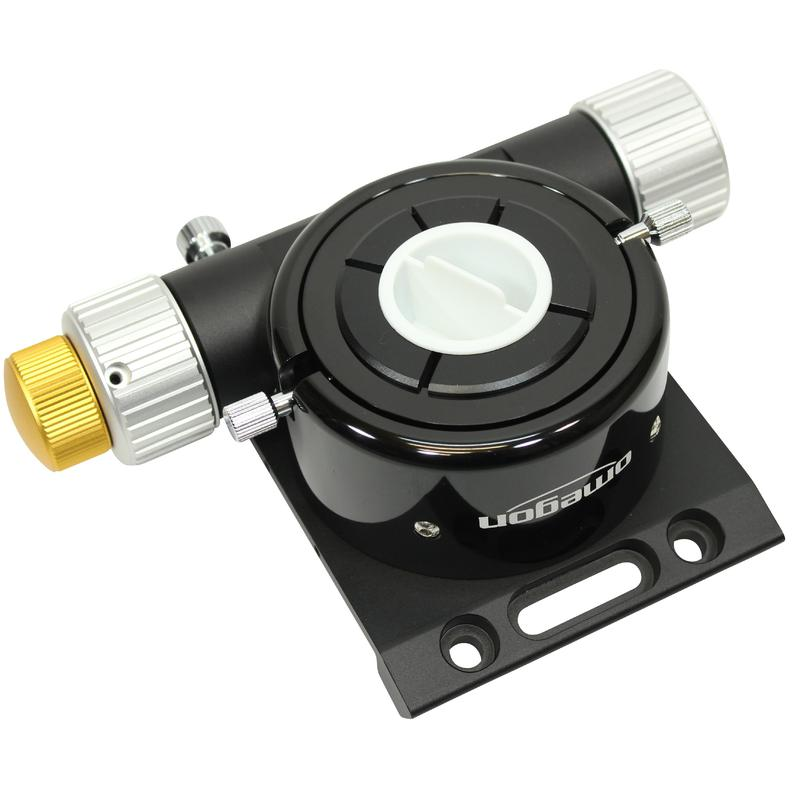
\includegraphics[width=1\textwidth]{../images/enfocador.jpg}
  \caption{Enfocador (\url{http://nimax-img.de/}).}
  \label{fig:diag_scrum}
  \end{center}
\end{figure}
http://cesar-programme.cab.inta-csic.es/

\bigskip
Un ejemplo de enfocador son los de tipo \textbf{Crayford} y los \textbf{rack and pinion}.

\subsection{Cúpulas}
Las \textbf{cúpulas} son recintos cerrados mas o menos grandes que nos permiten albergar y proteger el instrumental astronómico. De esta forma, las \textbf{cúpulas} pueden ser abiertas o cerradas para exponer los instrumentos en el momento de las observaciones.

\bigskip
\begin{figure}[!ht]
  \begin{center}
  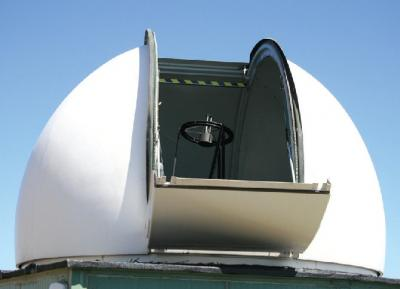
\includegraphics[width=1\textwidth]{../images/cupula.jpg}
  \caption{Cúpula (\url{http://cesar-programme.cab.inta-csic.es/}).}
  \label{fig:diag_scrum}
  \end{center}
\end{figure}
https://www.valkanik.com

\subsection{Ópticas activas/adaptativas}

La \textbf{óptica adaptativa} es una técnica que permite corregir las perturbaciones más importantes que sufren las imágenes astronómicas debido a la atmósfera terrestre. Con este sistema es posible obtener imágenes más nítidas o de mejor resolución espacial. La diferencia que introduce esta técnica es comparable a la que existe entre mirar un objeto situado en el fondo de una piscina con agua o sin agua.

\bigskip
\begin{figure}[!ht]
  \begin{center}
  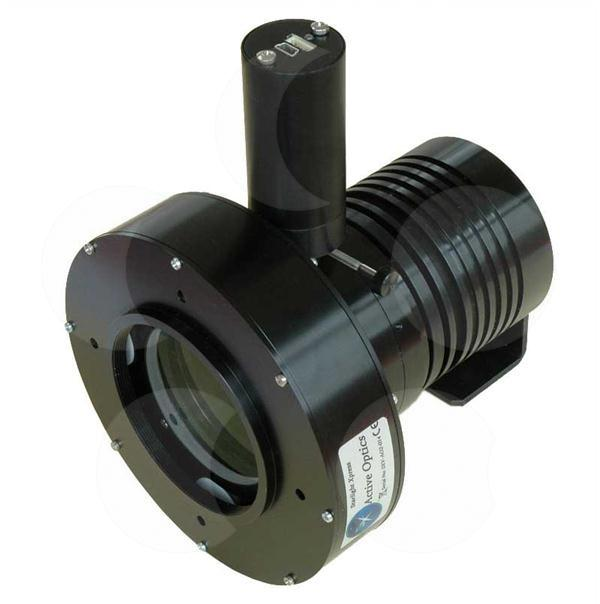
\includegraphics[width=1\textwidth]{../images/optica.jpg}
  \caption{Óptica adaptativa (\url{https://www.valkanik.com}).}
  \label{fig:diag_scrum}
  \end{center}
\end{figure}
http://www.depositohidrografico.com/


\bigskip
Las posibilidades que la óptica adaptativa ofrece a la astronomía son espectaculares. Eliminar las perturbaciones producidas por la atmósfera equivale esencialmente a observar desde el espacio. Las perturbaciones atmosféricas causan una pérdida en nitidez o resolución espacial. Esta pérdida se traduce, por un lado, en una disminuida capacidad para resolver objetos, es decir, para realizar estudios detallados de su morfología. Por otro lado, influye también en la capacidad de detectar objetos débiles, dado que la imagen se dispersa en puntos de luz mayores.

\bigskip
La mejora que introduce la óptica adaptativa se puede cuantificar utilizando la relación entre el tamaño del telescopio y el tamaño de la mejor imagen que puede obtener. El poder de detección de un telescopio aumenta con el diámetro de su espejo primario y disminuye con el tamaño de la imagen que forma de un objeto puntual (de aquí la importancia de la calidad de imagen en un telescopio). Por tanto, la diferencia con un mismo espejo de 10 metros, entre conseguir enfocar imágenes de 0.4 segundos de arco (lo posible en una noche de visibilidad excelente) y una imagen de 0.04 segundos de arco, que debe ser posible con un sistema de óptica adaptativa, equivaldría a tener un espejo primario de 100 metros

\subsection{Estaciones meteorológicas}

Las \textbf{estaciones meteorológicas} son sistemas compuestos por un \textit{``data logger''} y un conjunto de sensores que nos proprcionan datos de las distintas magnitudes meteorológicas, tales como la temperatura, humedad, presión barométrica, etc... permitiéndonos generar modelos a partir de los cuales conocer la situación climática y su posible evolución. 

\bigskip
\begin{figure}[!ht]
  \begin{center}
  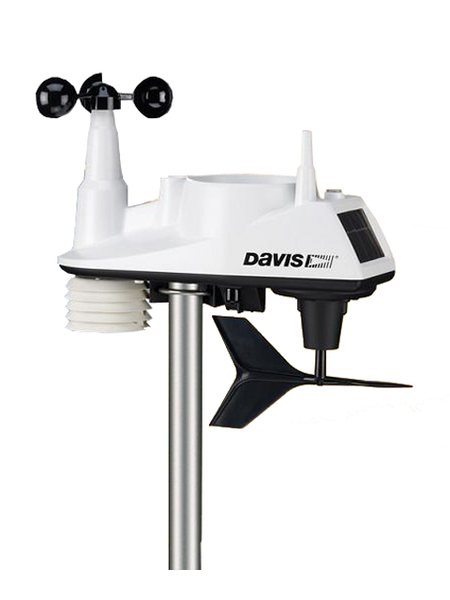
\includegraphics[width=1\textwidth]{../images/estacion.jpg}
  \caption{Estación meteorológica (\url{http://www.depositohidrografico.com/}).}
  \label{fig:diag_scrum}
  \end{center}
\end{figure}


\bigskip
Gracias a los datos aportados por las \textbf{estaciones meteorológicas}, podemos conocer la climatología en el momento de realizar observaciones astronómicas. De esta forma podemos decidir si las condiciones son óptimas, o incluso decidir si debemos cerrar la cúpula para evitar daños en los intrumentos por lluvias o similar. 

\newpage
\section{Control de dispositivos astronómicos}

Actualmente existen diversas formas de controlar los dispositivos astronómicos pero la mayoría presenta los mismos incovenientes:

\begin{itemize}
  \item Normalmente se controlan los dispositivos directamente.
  \item Se conecta el dispositivo a un PC y se trabaja desde él.
  \item Se utilizan herramientas para el control remoto como el \textif{``escritorio remoto''}.
\end{itemize}

\bigskip

Por otro lado, existen estándares como el de \textbf{ASCOM} para instrumental astronómico. Con él, se intenta crear una capa entre los programas para controlar dispositivos astronómicos y los propios dispositivos. \textbf{ASCOM} solo puede utilizarse en sistemas \textit{Microsoft Windows}. Su diseño tiene una relación bastante profunda con el sistema operativo lo cual dificulta el desarrollo basado en red.

\bigskip
\begin{figure}[!ht]
  \begin{center}
    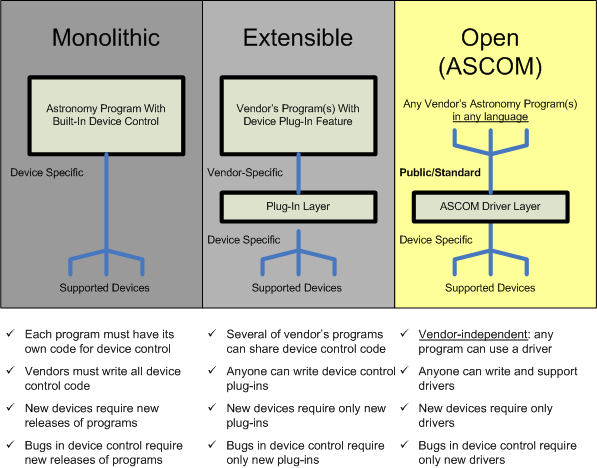
\includegraphics[scale=0.5]{../images/ascom.png}
    \caption{ASCOM Standard (\url{http://ascom-standards.org/})}
    \label{fig:ascom}
  \end{center}
\end{figure}


\newpage
\section{INDI}

\begin{quote}``\textit{The Instrument Neutral Distributed Interface (INDI) Library is a cross-platform software designed for automation & control of astronomical instruments. It supports a wide variety of telescopes, CCDs, focusers , filter wheels..etc, and it has the capability to support virtually any device. INDI is small, flexible, easy to parse, and scalable. It supports common DCS functions such as remote control, data acquisition, monitoring, and a lot more. With INDI, you have a total transparent control over your instruments so you can get more science with less time.}''
\newline(\url{http://indilib.org/about.html})
\end{quote}

\bigskip

El protocolo \textbf{INDI} es una plataforma software diseñada para el control de instrumental astronómico. La biblioteca \textbf{INDI} permite controlar cualquier dispositivo con un driver \textbf{INDI} mediante el paso de archivos XML. Sus principales ventajas frente a otras soluciones para el control de dispositivos son:


\begin{itemize}
  \item Es una biblioteca ligera, flexible y escalable.
  \item Es de código abierto por lo que cualquiera puede ver su código y mejorarlo o crear drivers para cualquier dispositivo
  \item El intercambio de información es mínimo.
  \item Es multiplataforma.
  \item Separa el cliente del servidor.
  \item Los fabricantes comienzan a desarrollar drivers para sus dispositivos o liberan las especificaciones para que la comunidad pueda desarrollarlos.
  \item Existen numerosos clientes INDI como \url{https://edu.kde.org/kstars/}

\end{itemize}

\bigskip
\begin{figure}[!ht]
  \begin{center}
    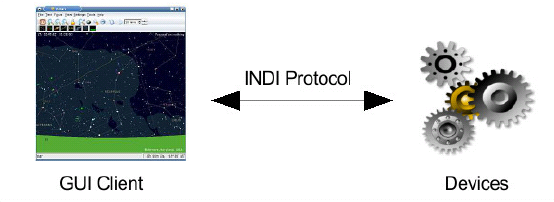
\includegraphics[width=1\textwidth]{../images/Indi_client.png}
    \caption{INDI Client (\url{http://www.indilib.org/})}
    \label{fig:indi_client}
  \end{center}
\end{figure}

\bigskip
\begin{figure}[!ht]
  \begin{center}
    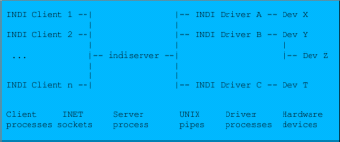
\includegraphics[width=1\textwidth]{../images/Indi_server.png}
    \caption{INDI Server (\url{http://www.indilib.org/})}
    \label{fig:indi_server}
  \end{center}
\end{figure}

\bigskip

\subsection{Breve introducción a INDI}

INDI consiste a su nivel más básico en un protocolo que permite el control, automatización, obtención de datos e intercambio de los mismos entre distintos dispositivos hardware y programas cliente. La idea subyacente en el protocolo INDI es desacoplar aspectos específicos del hardware que se controla de tal manera que cambios en el hardware no impliquen necesariamente cambios en el software (cosa que ocurre en sistemas más habituales donde el el frontend software está fuertemente acoplado con el backend hardware.

\bigskip
Para conseguir un desacople efectivo entre los clientes y el hardware se define un protocolo basado en XML que permite abstraer los dispositivos hardware como conjuntos de propiedades que pueden ser leidas, y modificadas por los clientes (siempre estableciendo las restricciones oportunas).


\subsection{Drivers, Servidores y Clientes INDI}

Pese a que nivel más básico INDI es ``simplemente'' una especificación de un protocolo basado en XML, a un nivel superior se distinguen tres entidades diferentes que interaccionan entre sí para tener un sistema de control plenamente funcional:

\begin{itemize}
  \item \textbf{Drivers:} Son programas que se ejecutarán en la máquina en la que están conectados los dispositivos hardware. Son los encargados de la comunicación directa con los dispositivos y su abstracción a propiedades INDI.
  
  \item \textbf{Servidor:} Es un programa cuya función principal es ejecutar los drivers y permitir la conexión a los mismos por parte de los clientes (funciona de un modo similar a un proxy). Normalmente reside en la máquina donde están conectados los dispositivos, aunque en principio se pueden crear estructuras de red tipo árbol de servidores. El interambio de información entre el servidor y los drivers se realiza utilizando el protocolo INDI.
  
  \item \textbf{Cliente:} Es un programa que permite conectar con uno o más servidores y su función principal e hacer de interfaz con el usuario. Para ello conecta (usualmente a través de la red) con el servidor e intercambia información sobre los dispositivos utilizando el protocolo INDI (FIGURA \ref{fig:indi_server} ). Es interesante recalcar que los clientes pueden ser de cualquier estilo: desde programas con interfaz de usuario avanzadas, hasta programas simples en línea de comandos scripts completamente automáticos que controlen o monitoricen los dispositivos.
\end{itemize}


\subsection{Abstracción de los Dispositivos}

Para conseguir abstraer los dispositivos y que puedan ser controlados o monitorizados por los clientes el protocolo INDI define las llamadas \textit{propiedades}. Las propiedades tienen ciertas características como por ejemplo:

\begin{itemize}
  \item \textbf{Permiso:} Las propiedades tienen uno de 3 posibles permisos:
    \begin{itemize}
     \item \textbf{Lectura y escritura (R/W):} La propiedad puede ser leida y modificada.
     \item \textbf{Solo lectura (RO)}
     \item \textbf{Solo escritura (WO)}
    \end{itemize}

  \item \textbf{Estado:} Las propiedades tienen uno de los siguientes 4 posibles estados:
    \begin{itemize}
     \item \textbf{Ok:} Estado correcto
     \item \textbf{Idle:} Estado indefinido (normalmente la propiedad aun no ha sido usada)
     \item \textbf{Busy:} Está ocupada (probablemente cambiando de valor)
     \item \textbf{Alert:} Ha ocurrido algún problema con la propiedad.
    \end{itemize}
\end{itemize}

\bigskip
Al margen de esas características, hay que mencionar que las propiedades son un conjunto de usualmente uno o más elementos distintos. Es decir, una única propiedad puede agregar varios valores distintos (normalmente relacionados).

Existen 5 tipos de propiedades distintas:

\begin{itemize}
 \item \textbf{Textuales:} Permiten manejar información textual (cadenas de caracteres).
 
 \item \textbf{Numéricas:} Permiten manejar información numérica. Estas propiedades permiten espeificar los rangos de valores válidos así como el formato de visualización del número (entero, flotante, flotante exponencial o sexagesimal).
 
 \item \textbf{Luces:} Permiten manejar ``señales'' o luces que tienen uno de los siguientes cuatro posibles valores:
   \begin{itemize}
     \item \textbf{Ok}
     \item \textbf{Idle}
     \item \textbf{Busy}
     \item \textbf{Alert}
   \end{itemize}


 \item \textbf{Switch:} Permiten manejar valores entre una lista de posibles alternativas. Permiten especificar la regla de selección de cada una de las alternativas:
   \begin{itemize}
     \item \textbf{Una de muchas:} De todas las alternativas, una y solo una debe estar elegida.
     \item \textbf{Como mucho una:} De todas las alternativas se puede elegir una o ninguna.
     \item \textbf{Cualesquiera de muchas:} De todas las alternativas se pueden seleccionar cualquier numero de ella (desde ninguna a todas).

   \end{itemize}
 \item \textbf{BLOB:} Permite manejar valores binarios (como por ejemplo datos de imagen en una cámara).

\end{itemize}



\subsection{Ejemplo de Abstracción de un Dispositivo}

Para comprender mejor el mecanismo de abstracción que aplica INDI, vamos a realizar un ejemplo sencillo de como el programador de un driver abstrae un dispositivo. Supongamos que se trata de una cámara sencilla. La especificación de la cámara dice que su funcionamiento es muy simple: Solo hace falta comunicarle por el puerto serie un comando que incluye el tiempo de exposición de la misma. Una vez mandado ese comando la cámara tomará la fotografía y devolverá los datos de la fotografía en bruto, como un array de valores numéricos (a mayor valor, mayor intensidad luminosa del pixel).

\bigskip
Por tanto, para ofrecer la funcionalidad al cliente INDI, el driver define las siguientes propiedades:

\begin{itemize}
  \item \texttt{Nombre del driver:} Tipo texto, \texttt{RO}. Contendrá el nombre del driver y dispositivo. No cambiará nunca.
  \item \texttt{Tiempo de Exposición:} Tipo numérico, \texttt{R/W}, entre \texttt{0} y \texttt{3600} (segundos). Por defecto \texttt{0}.
  \item \texttt{Imagen:} Tipo BLOB, \texttt{RO}. Contendrá la información binaria de la imagen. En este ejemplo, será una imagen tipo \texttt{PNG}.
\end{itemize}

\bigskip
El driver, además de definir esas propiedades tendrá el siguiente comportamiento general:

\begin{itemize}
 \item Cuando conecte un cliente mandará la información de las tres propiedades.
 \item Quedará a la espera de que cambie el \texttt{tiempo de exposición}.
 \item Cuando el cliente mande un \texttt{tiempo de exposición} nuevo, mandará el comando apropiado a la cámara para que haga la captura de la imagen y esperará a recibir los datos binarios en bruto de la misma.
 \item Una vez recibidos dichos datos binarios los transformará a formato  \texttt{PNG}.
 \item Mandará al cliente nuevos valores para las propiedades de \texttt{tiempo de exposición} (\texttt{0}, para indicar que ya ha acabado la exposición) e \texttt{imagen} (con los datos binarios, el \texttt{PNG}).
\end{itemize}

\subsection{INDI for Java}

La biblioteca \textbf{INDI} está escrita en lenguaje \textbf{C}, pero existe una implementación realizada en Java y que se encuentra en desarrollo. En la página oficial de \textbf{INDI} \url{http://indilib.org/develop/indiforjava.html} podemos encontrar toda la información sobre nuevas versiónes y la documentación para poder utilizarla. La principal ventaja de poder usar Java es que podemos implementar drivers y clientes con la potencia de un lenguaje Orientado a Objetos y combinarlo con otras tecnologías como los dispositivos móviles basados en la plataforma \textbf{Android}


\newpage

\section{Dispositivos Móviles}

Un \textbf{dispositivo móvil} es un tipo de computadora de tamaño pequeño, con capacidad de procesamiento, con conexión a internet, con memoria, diseñados especifcamente para una función pero que pueden llevar a cabo otras funciones más generales.

\bigskip
Los \textbf{dispositivos móviles} hoy en día están integrados en la mayoría de tareas cotidianas de una persona. La tendencía de la sociedad actual nos empuja hacia un mundo cada vez más móvil donde necesitamos estar conectado e interactuar con otros sitemas. Es por ello que la mayoría de soluciones tecnológicas, hayan sido pensadas o no para el sector de los dispositivos móviles, siempre acaba teniendo una versión para éstos.

\bigskip
Paralelamente a la expansión de los \textbf{dispositivos móviles}, se han creado un gran número de sistemas operativos para estos dispositivos entre los que se encuentra:

\begin{itemize}
  \item Android.
  \item iOS.
  \item BlackBerry OS.
  \item Palm OS.
  \item Windows Mobile/Phone.
  \item Symbian.
\end{itemize}

\bigskip
Actualmente \textbf{Android} y \textbf{iOS} copan el 96.3\% del mercado\footnote{Fuente:http://www.idc.com/getdoc.jsp?containerId=prUS25450615.} . Por lo que nos centraremos principalmente en estos sistemas operativos (S.O.) y los \textbf{dispositivos móviles} compatibles con ellos.

\subsection{iOS}

\textbf{iOS} es un S.O. móvil de la compaía \textit{Apple Inc} originalmente desarrollado para el \textit{iPhone}\footnote{Smartphone de la compañia Apple Inc.} y posteriormente introducido en otros \textbf{dispositivos móviles} de la compañía como el iPod touch\footnote{Dispositivo móvil para reproducir multimedia de la compañía Apple Inc} y el iPad\footnote{Tablet de la compañía Apple Inc.}. \textbf{iOS} no puede ser instalado en hardware de terceros.

\bigskip
Actualmente tiene una cuota de mercado aproximadamente del 19.7\%, siendo el segundo S.O. más utilizado.

\bigskip
\textbf{iOS} es un sistema muy estable, diseñado para un hardware muy concreto y por tanto, muy eficiente y depurado. Pero de cara a elegirlo como una opción a la hora de desarrollar una nueva aplicación para \textbf{dispositivos móviles} se debe tener en cuenta los siguientes aspectos:

\begin{itemize}
  \item Hay que pagar una cuota anual de 99\$ para poder publicar aplicaciones en el \textit{Apple Store}\footnote{Tienda de aplicaciónes de la compañia Apple Inc.}. Además si esta licencia, no podremos desarrollar aplicación y cargarla en nuestros dispositivos Apple.
  \item Necesitamos un MAC\footnote{Computadoras personales de la compañia Apple Inc.} ya que las herramientas para el desarrollador solo pueden utilizarse en sus equipos.
  \item Necesitaremos conocer el lenguaje de programación \textbf{Objective-C}
  \item \textbf{iOS} es un sistema de código cerrado que va en contra de la filosofía del \textbf{Software Libre} y el código abierto y reutilizable.

\end{itemize}

\bigskip
Aunque \textbf{iOS} es un sístema muy extendido y con un gran número de usuarios, creemos que no es la mejor opción para orientar una aplicación móvil basada en \textbf{Software Libre} además de la inversión anual requerida para poder publicar una aplicación que prendemos sea gratuita, libre y accesible a cualquier usuario.


\subsection{Android}

\textbf{Android} es un Sistema Operativo basado en un \textbf{núcleo Linux}\footnote{Sistema operativo basado en Unix}. Fue diseñado principalmente para dispositivos móviles con pantalla táctil, relojes inteligentes, televisiones inteligentes y automóviles. Inicialmente pertenecía a la compañía \textbf{Android Inc.} que posteriormente sería adquirida por \textbf{Google}. Actualmente posee la mayor cuota de mercado de aproximadamente el 76.6\%.

\bigskip
Los principales componentes del sistema operativo \textbf{Android} son:


\begin{itemize}
  \item \textbf{Aplicaciones}: Todas las aplicaciones están escritas en lenguaje de programación \textbf{Java}.
  \item \textbf{Framework}\footnote{Marco de trabajo para los desarrolladores}: Los desarrolladores tiene acceso completo a las mismas API's\footnote{Interfaz de programación de aplicaciones (Application Programming Interface)} que utiliza el sistema. La arquitectura está diseñada para simplificar la reutilización de componentes.
  \item \textbf{Runtime de Android}: Adroid incluye un set de bibliotecas base que porporcionanla mayor parte de las funciones disponibles en las bibliotecas base del lenguaje \textbf{Java}. Cada aplicación android corre su propio proceso, con su propia instancia de la máquina virtual \textit{Dalvik}\footnote{Máquina virtual que utiliza la plataforma Android para ejecutar aplicaciones Java.}
  \item \textbf{Núcleo Linux}: Android depende de Linux para los servicios base del sistema como la seguridad, la gestión de memoria, la gestión de procesos, etc. El núcleo Linux también sirve como capa de abstracción entre el hardware y el software.
\end{itemize}

\bigskip
\textbf{Android} no tiene restricciones de uso por lo que puede utilizarse en número muy extenso de dispositivos móviles. Además es un sistema parcialmente de código abierto. Está basado en Linux y la mayoría del código es abierto aunque no todo el sistema lo es.

\bigskip
De cara al desarrollo de aplicaciones móviles, \textbf{Android} es una opción muy recomendable por las siguientes razones:

\begin{itemize}
  \item La arquitectura del sistema (basada en Linux, lenguaje de programación Java,...)
  \item La mayoría de los dispositivos móviles del mundo tienen como sistema operativo a \textbf{Android} por lo que la difusión será mayor que con otros sistemas.
  \item Las herramientas para desarrollar en Android son multiplataforma y gratuitas. Para poder crear y probar una aplicación solo necesitas un ordenador con cualquier sistema operativo, un dispositivo móvil con android y descargar la herramienta para desarrolladores.
  \item Para poder publicar aplicaciones en \textit{Google Play}\footnote{Tienda de aplicaciones para dispositivos Android} hay que pagar 25\$ sin tener renovarlo anualmente y sin ninguna limitación.
\end{itemize}